\documentclass[../main.tex]{subfiles}
\graphicspath{{\subfix{../images/}}}
\begin{document}
\section*{Term 1 Week 10}
\begin{enumerate}
    \item 
    Using Pythagoras, we get the lengths of the diagonal into the centre of the large square:\\
    \(d=\sqrt{2^+2^2}=\sqrt{8}=2\sqrt{2}\)
    \begin{figure}[H]
        \centering
        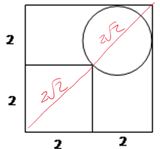
\includegraphics[width=0.2\linewidth]{images/t1w10q1_a1.png}
    \end{figure}
    Form a right-angle triangle at the centre of the circle, with side lengths of \(r, r \text{and} 2\sqrt{2}-r\):
    \begin{figure}[H]
        \centering
        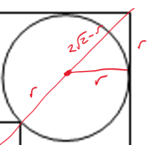
\includegraphics[width=0.2\linewidth]{images/t1w10q1_a2.png}
    \end{figure}

    Use Pythagoras again:\\
    \(r^2 + r^2=(2\sqrt{2}-r)^2\)\\
    \(2r^2=8-4\sqrt{2}r+r^2\)\\
    \(r^2+4\sqrt{2}r-8=0\)\\
    Solving for r:\\
    \(r=\frac{-4\sqrt{2}\pm \sqrt{32-4\times 1\times -8}}{2}\)\\
    \(r=\frac{-4\sqrt{2}\pm 8}{2}\)\\
    \(r=4-2\sqrt{2}, -4-2\sqrt{2}\)\\
    Since the radius must be positive, \(r=4-2\sqrt{2}\)\\

    \textit{Alex Manson's approach}:\\
    \begin{figure}[H]
        \centering
        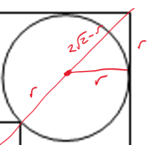
\includegraphics[width=0.2\linewidth]{images/t1w10q1_a2.png}
    \end{figure}
    We know the length of the diagonal from the centre to the top-right is \(2\sqrt{2}\). We also know that from Pythagoras that the distance from the centre of the circle to the top-right corner is \(r\sqrt{2}\).\\
    This means that \(r+r\sqrt{2}=2\sqrt{2}\)\\
    \(r=\frac{2\sqrt{2}}{1+\sqrt{2}}\)\\
    \(r=\frac{2\sqrt{2}-4}{1-2}=4-2\sqrt{2}\)\\

    \textit{Jack Li's approach}:\\
    Using similar triangles:
    \begin{figure}[H]
        \centering
        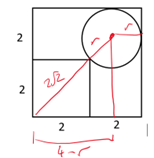
\includegraphics[width=0.2\linewidth]{images/t1w10q1_a3.png}
    \end{figure}
    By extending the diagonal through the centre of the square to the centre of the circle, we create two similar triangles. This gives us:\\
    \(\frac{2\sqrt{2}+r}{4-r}=\frac{2\sqrt{2}}{2}\)\\

    \(\frac{2\sqrt{2}+r}{4-r}=\sqrt{2}\)\\

    \(2\sqrt{2}+r=4\sqrt{2}-r\sqrt{2}\)\\

    \(r+r\sqrt{2}=2\sqrt{2}\)\\

    \(r=\frac{2\sqrt{2}}{1+\sqrt{2}}\)\\

    \(r=\frac{2\sqrt{2}}{1+\sqrt{2}}\times \frac{1-\sqrt{2}}{1-\sqrt{2}}=4-2\sqrt{2}\)\\
    
    \item 
    Use similar shapes and ratios. Triangle ABC is similar to EFC, meaning:\\
    \(\frac{8}{a+b}=\frac{x}{b}\)\\
    \(8b=(a+b)x\)\\

    Also, triangle ADC is similar to AFE, meaning:\\
    \(\frac{5}{a+b}=\frac{x}{a}\)\\
    \(5a=(a+b)x\)\\

    Equating the two, we get \(5a=8b\)\\
    \(b=\frac{5}{8}a\)\\

    Substituting into one of the equations:\\
    \(5a=(a+\frac{5}{8}a)x\)\\

    \(x=\frac{5a}{a+\frac{5}{8}a}=\frac{5a}{\frac{8a+5a}{8}}=\frac{5a}{\frac{13a}{8}}=\frac{40a}{13a}=\frac{40}{13}=3.08\)\\

    \item 
    Start by labelling angles A, B and C, and the opposite sides a, b and c:
    \begin{figure}[H]
        \centering
        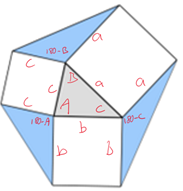
\includegraphics[width=0.25\linewidth]{images/t1w10q3_a.png}
    \end{figure}

    Now we can use the formula for area of a triangle to find the area of the grey triangle. It can be any of these three:\\
    \(A=\frac{1}{2}ab\sin{C}\)\\
    \(A=\frac{1}{2}ac\sin{C}\)\\
    \(A=\frac{1}{2}bc\sin{C}\)\\

    The area of each of the blue triangles will be:\\
    \(A=\frac{1}{2}ac\sin{(180-B)}\)\\
    \(A=\frac{1}{2}ab\sin{(180-C)}\)\\
    \(A=\frac{1}{2}bc\sin{(180-A)}\)\\

    Using the sine compound angle rule, we know that:\\
    \(\sin{(180-B)}=\sin{180}\cos{B}-\cos{180}\sin{B}=\sin{B}\)\\
    And so on for each of the blue triangles.\\
    Therefore, their areas are:\\
    \(A=\frac{1}{2}ac\sin{(B)}\)\\
    \(A=\frac{1}{2}ab\sin{(C)}\)\\
    \(A=\frac{1}{2}bc\sin{(A)}\)\\

    This means each of the blue triangles has the same area as the original, so their total area is 300\(\%\) of the original grey triangle.\\
    
    \item 
    Set V as the volume of the tank. Also set \textbf{x} as the constant volume per hour that the first outlet pipe drains the tank, \textbf{b} the constant volume per hour of the second outlet pipe, and \textbf{c} as the constant volume per hour of the third outlet pipe.\\
    Now we can set up equations for each situation:\\
    \(12(a+b)=V\\
    15(a+c)=V\\
    20(b+c)=V\)\\
    Now just solve simultaneously.\\
    \begin{equation}
        a+b=\frac{V}{12}
    \end{equation}
    \begin{equation}
       a+c=\frac{V}{15} 
    \end{equation}
    \begin{equation}
      b+c=\frac{V}{20}  
    \end{equation}
    Equation (1) - equation (2) gives \(b-c=\frac{V}{60}\)\\
    Then adding equation 3 gives:\\
    \(2b=\frac{V}{15}\)\\
    \(b=\frac{V}{30}\) Therefore, outlet pipe \textbf{b} takes 30 minutes to drain the tank.\\

    Substituting into equation 1 and equation 3 to get \textbf{a} and \textbf{c}:\\
    \(a+\frac{V}{30}=\frac{V}{12}\)\\
    \(a=\frac{V}{20}\) Therefore, outlet pipe \textbf{a} takes 20 minutes to drain the tank.\\

    \(\frac{V}{30}+c=\frac{V}{20}\)\\
    \(c=\frac{V}{60}\) Therefore, outlet pipe \textbf{c} takes 60 minutes to drain the tank.\\
    
    \textit{Alternative approach using common denominators:}\\
    If \textbf{a}, \textbf{b} and \textbf{c} were all turned on for 60 hours, \(a+b\) would empty the tank 5 times, \(a+c\) would empty it 4 times, and \(b+c\) would empty it 3 times. That is a total of 12.\\ However, in that time, \textbf{a}, \textbf{b} and \textbf{c} have run twice, so we know that \(2a+2b+2c\) empties the tank 12 times.\\
    \textbf{Important:} This means \(a+b+c\) would empty the tank 6 times.\\

    Now, we know that \(a+b\) empties the tank 5 times in 60 hours, therefore \textbf{c} would empty it once. This means \textbf{c} would take 60 hours to empty the tank.\\
    
    We know that \(a+c\) empties the tank 4 times in 60 hours, therefore \textbf{b} would empty it twice. This means \textbf{b} would take 30 hours to empty the tank.\\
    
    Finally, we know that \(b+c\) empties the tank 3 times in 60 hours, therefore \textbf{a} would empty it 3 times. This means it would take \textbf{a} 20 hours to empty the tank.

\end{enumerate}

\end{document}